\paragraph{QuizziPedia::Front-End::Controllers::HomeController}
\begin{figure} [ht]
	\centering
	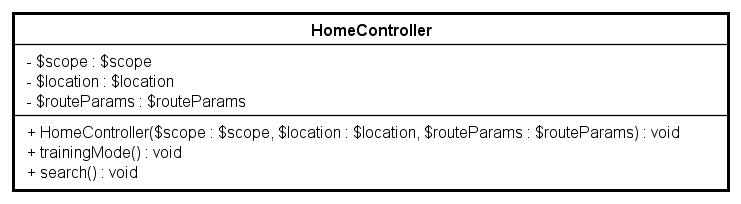
\includegraphics[scale=0.6]{UML/Classi/Front-End/QuizziPedia_Front-end_Controller_HomeController.png}
	\caption{QuizziPedia::Front-End::Controllers::HomeController}
\end{figure} \FloatBarrier
\begin{itemize}
	\item \textbf{Descrizione}: questa classe permette di gestire la home page;
	\item \textbf{Utilizzo}: fornisce tutte le informazioni da mostrare nella homepage;
	\item \textbf{Relazione con altre classi}:
	\begin{itemize}
		\item \textbf{IN} \texttt{HomeModelView}: classe di tipo modelview la cui istanziazione è contenuta all'interno della variabile di ambiente \$scope di \textit{Angular.js\ped{G}}. All'interno di essa sono presenti le variabili e i metodi necessari per il \textit{Two-Way Data-Binding\ped{G}} tra la \textit{view\ped{G}} \texttt{HomeView} e il \textit{controller\ped{G}} \texttt{HomeController};
	\end{itemize}
	\item \textbf{Attributi}:
	\begin{itemize}
		\item \texttt{-} \texttt{\$scope: \$scope} \\
		Campo dati contenente un riferimento all'oggetto \$scope creato da \textit{Angular\ped{G}}, viene utilizzato come mezzo di comunicazione tra il \textit{controller\ped{G}} e la \textit{view\ped{G}}. Contiene gli oggetti che definiscono il \textit{model\ped{G}} dell'applicazione;
		\item \texttt{-} \texttt{\$location: \$location} \\
		Campo dati contenente un riferimento al servizio creato da \textit{Angular\ped{G}} che permette di accedere alla barra degli indirizzi del \textit{browser\ped{G}}, i cambiamenti all'URL nella barra degli indirizzi si riflettono in questo oggetto e viceversa.
	\end{itemize}
	\item \textbf{Metodi}:
	\begin{itemize}
		\item \texttt{+} \texttt{HomeController(\$scope: \$scope, \$location: \$location)} \\
		Metodo costruttore della classe: \\
		\textbf{Parametri}:
		\begin{itemize}
			\item \texttt{\$scope: \$scope} \\
			Parametro contenente un riferimento all'oggetto \$scope creato da \textit{Angular\ped{G}}. Viene utilizzato come mezzo di comunicazione tra il \textit{controller\ped{G}} e la \textit{view\ped{G}}. Contiene gli oggetti che definiscono il viewmodel e il \textit{model\ped{G}} dell'applicazione;
			\item \texttt{\$location: \$location} \\
			Parametro contenente un riferimento al servizio creato da \textit{Angular\ped{G}} che permette di accedere alla barra degli indirizzi del \textit{browser\ped{G}}, i cambiamenti all'URL nella barra degli indirizzi si riflettono in questo oggetto e viceversa.
		\end{itemize}
		\item \texttt{+} \texttt{trainingMode(): void} \\
		Metodo che gestisce l’evento click sul pulsante di allenamento. Effettua il redirect alla pagina di allenamento.
	\end{itemize}
\end{itemize}

